\section{overall themes}
\begin{frame}<1>[label=themes]{themes}
\begin{itemize}
    \item \myemph<2>{automating building software}
        \begin{itemize}
        \item libraries, taking advantage of incremental compilation
        \end{itemize}
    \item \myemph<3,4,5>{sharing machines}
        \begin{itemize}
        \item multiple users/programs on one system
        \end{itemize}
    \item \myemph<4>{parallelism and concurrency}
        \begin{itemize}
        \item doing two+ things at once
        \end{itemize}
    \item \myemph<6>{under the hood of sockets}
        \begin{itemize}
        \item layered design of networks
        \item implementing secure communication
        \end{itemize}
    \item \myemph<7>{under the hood of fast processors}
        \begin{itemize}
        \item caching, (hidden) parallelism, avoiding idle time
        \end{itemize}
    \end{itemize}
\end{frame}

\themesSlide{1}

\section{briefly, building}
\themesSlide{2}

\begin{frame}[fragile]{make}
\begin{Verbatim}
$ ./foo.exe
...
...
$ edit readline.c
$ make
clang -g -O -Wall -c readline.c -o readline.o
ar rcs terminal.o readline.o libreadline.a
clang -o foo.exe libreadline.a foo.o foo-utility.o bar.o
$ 
\end{Verbatim}
\end{frame}


\section{briefly, virtual memory}

\themesSlide{3}

\usetikzlibrary{arrows.meta,calc,positioning,shapes.multipart}
\begin{frame}{address translation}
\myalttext{
\begin{tikzpicture}
\tikzset{
    every node/.style={font=\small},
}
\node[align=center,alt=<2>{draw=red,very thick,fill=red!10}{}] (progAAddr) {Process A \\ addresses \\ \myemph<3>{``virtual''}};
\begin{visibleenv}<2>
\node[align=left,below=.5cm of progAAddr] {\myemph{every address accessed} \\ instructions \textit{and} data};
\end{visibleenv}
%\node[below=1cm of progAAddr,align=center] (progBAddr) {Process B \\ addresses};
\node[draw, right=3cm of progAAddr,align=center,alt=<4>{draw=red,very thick,fill=red!10}] (translationA) { mapping \\ (set by OS) };
\begin{visibleenv}<4>
\node[align=left,below=.5cm of translationA] {stored in processor? \\ format?};
\end{visibleenv}
%\node[draw, right=3cm of progBAddr,align=center] (translationB) { mapping \\ (set by OS) };
\node[draw,rectangle split, rectangle split parts=6, anchor=north west,label={[align=center]north:real memory\\\myemph<3>{``physical''}}] (mem) at ([xshift=3cm]translationA.north east) {
    \nodepart{one}
    Process A code 
    \nodepart{two}
    Process B code
    \nodepart{three}
    Process A data
    \nodepart{four}
    Process B data
    \nodepart{five}
    OS data
    \nodepart{six}
    \ldots
};
\draw[-Latex,green,thick] (progAAddr) -- (translationA) (translationA.east) -- (mem.one west);
\draw[-Latex,green,thick] (translationA.east) -- (mem.three west);
%\draw[-Latex,blue,thick] (progBAddr) -- (translationB) (translationB.east) -- (mem.two west);
%\draw[-Latex,blue,thick] (translationB.east) -- (mem.four west);
%\node[thick,red,draw,anchor=north west] (error) at ([yshift=-.5cm]mem.south west) {trigger error};
%\draw[-Latex,green,thick] (translationA.east) -- (error.west);
%\draw[-Latex,blue,thick] (translationB.east) -- (error.west);
%\draw[-Latex,green,ultra thick,dotted] (translationA.east) -- (mem.five west);
%\draw[-Latex,blue,ultra thick,dotted] (translationB.east) -- (mem.five west);
\begin{visibleenv}<3>
\node[draw,thick,align=center,below=3cm of translationA] {
    program addresses are `virtual' \\
    real addresses are `physical' \\
    can be \myemph{different sizes}!
};
\end{visibleenv}
\end{tikzpicture}
}{%
    Diagram showing program addresses (program and data) being converted to real addresses using a mapping set by the OS.
    The program addresses are called "virtual" and the real addresses are called "physical".
}
\end{frame}


\usetikzlibrary{arrows.meta,fit}

\begin{frame}{address spaces}
\begin{itemize}
\item illusion of \myemph{dedicated memory}
\end{itemize}
\myalttext{
\begin{tikzpicture}
\tikzset{
    every node/.style={font=\small},
}
\node[align=center] (progAAddr) {Process A \\ addresses};
\node[below=1cm of progAAddr,align=center] (progBAddr) {Process B \\ addresses};
\node[draw, right=3cm of progAAddr,align=center] (translationA) { mapping \\ (set by OS) };
\node[draw, right=3cm of progBAddr,align=center] (translationB) { mapping \\ (set by OS) };
\node[draw,rectangle split, rectangle split parts=6, anchor=north west,label={north:real memory}] (mem) at ([xshift=3.5cm]translationA.north east) {
    \nodepart{one}
    Process A code 
    \nodepart{two}
    Process B code
    \nodepart{three}
    Process A data
    \nodepart{four}
    Process B data
    \nodepart{five}
    OS data
    \nodepart{six}
    \ldots
};
\draw[-Latex,green,thick] (progAAddr) -- (translationA) (translationA.east) -- (mem.one west);
\draw[-Latex,green,thick] (translationA.east) -- (mem.three west);
\draw[-Latex,blue,thick] (progBAddr) -- (translationB) (translationB.east) -- (mem.two west);
\draw[-Latex,blue,thick] (translationB.east) -- (mem.four west);
\node[thick,draw,anchor=north west] (error) at ([yshift=-.5cm]mem.south west) {trigger exception};
\draw[-Latex,green,thick] (translationA.east) -- (error.west);
\draw[-Latex,blue,thick] (translationB.east) -- (error.west);
\draw[-Latex,green,ultra thick,dotted] (translationA.east) -- (mem.five west);
\draw[-Latex,blue,ultra thick,dotted] (translationB.east) -- (mem.five west);
\draw[-Latex,ultra thick,dotted] ([xshift=-3cm,yshift=-.5cm]translationB.south) -- ([xshift=-2cm,yshift=-.5cm]translationB.south)
    node[right] {= kernel-mode only};
\begin{visibleenv}<2>
    \node[fill=red,fill opacity=0.1,draw=red,ultra thick,fit=(translationA) (translationB),label={[red]north:chose one during context switch}] {};
\end{visibleenv}
\end{tikzpicture}
}{Diagram showing processes A and B have different mappings from virtual (program) to physical (real) addresses set by the OS.
The mapping can also specifies that some addresses trigger exceptions or are usable in kernel mode only.}
\end{frame}


\subsection{interrupts}

\themesSlide{4}

\usetikzlibrary{patterns}

\begin{frame}{keyboard input timeline}
\begin{tikzpicture}
\tikzset{
    prog1/.style={draw,fill=cyan},
    prog2/.style={draw,fill=green},
    prog3/.style={draw,fill=violet!30},
    proglabel/.style={font=\tt\scriptsize},
    labelprog1/.style={execute at begin node={\strut },pin={south:\tt\scriptsize read\_input.exe}},
    labelprog2/.style={execute at begin node={\strut }},
    labelprog3/.style={execute at begin node={\strut }},
}
\begin{scope}[xscale=1.5,yscale=1]
\foreach \s/\e/\p [count=\x] in {0/0.5/1,0.5/3/2,3/5.4/3,5.4/7/1} {
    \coordinate (s-\x) at (\s, 0);
    \coordinate (e-\x) at (\e, 0);
    \draw[prog\p] (\s, 0) rectangle (\e, 1) coordinate[midway] (mid-\x);
    \node[anchor=center,proglabel,labelprog\p] at (mid-\x) {};
    \begin{pgfonlayer}{fg}
    \draw[fill=white] ([xshift=-.05cm]e-\x) rectangle ([xshift=.05cm,yshift=1cm]e-\x);
    \draw[pattern=north west lines] ([xshift=-.05cm]e-\x) rectangle ([xshift=.05cm,yshift=1cm]e-\x);
    \end{pgfonlayer}
}
\end{scope}
% FIXME: mark types of exceptions at each transition
\draw[red,very thick,Latex-] ([xshift=-.05cm]e-1) -- (2, -3) node[fill=white,draw] {trap --- {\tt read} system call};
\draw[red,very thick,Latex-] ([xshift=-.05cm]e-3) -- (7, -4) node[fill=white,draw] {interrupt --- from keyboard};
\begin{scope}[xshift=2cm]
\draw[fill=white,pattern=north west lines] (0, -1) rectangle (1, -2);
\node[anchor=west] at (1, -1.5) {\strut = operating system};
\end{scope}
\end{tikzpicture}
\end{frame}




\usetikzlibrary{arrows.meta}

\begin{frame}[fragile,label=timeMulti1]{time multiplexing}
\begin{tikzpicture}
\tikzset{
    prog1/.style={draw,fill=cyan!70},
    prog2/.style={draw,fill=green,visible on=<3->},
    prog3/.style={draw,fill=violet!30,visible on=<3->},
    proglabel/.style={font=\tt\scriptsize},
    labelprog1/.style={execute at begin node={\strut loop.exe}},
    labelprog2/.style={execute at begin node={\strut ssh.exe},visible on=<3->},
    labelprog3/.style={execute at begin node={\strut firefox.exe},visible on=<3->},
}

\begin{scope}[xscale=1.5,yscale=1]
\foreach \s/\e/\p [count=\x] in {0/2/1,2/3/2,3/5/3,5/6/1,6/7/2}{
    \draw[prog\p] (\s, 0) rectangle (\e, 1) coordinate[midway] (mid-\x);
    \node[anchor=center,proglabel,labelprog\p] at (mid-\x) {};
}
\end{scope}
\node[anchor=east] at (-0.25, 0.5) {CPU:};
% FIXME: system
\begin{scope}[yscale=1,yshift=-2.5mm]
\draw[thick,-Latex] (1,0) node[left] {time} -- (10.5,0);
\end{scope}
\begin{visibleenv}<2->
    \begin{scope}[xscale=1.5]
    \draw[red,thick] (1.9,-.1) coordinate (firstStart) rectangle (2.0, 1.1);
    \draw[red,thick] (5.1,-.1) coordinate (lastEnd) rectangle (5.0, 1.1);
    \end{scope}
    \node[anchor=north west] (asmPre) at (0, -1) {
\begin{lstlisting}[language=myasm,style=small]
...
call get_time 
    // whatever get_time does
movq %rax, %rbp
\end{lstlisting}
    };
    \draw[red, ultra thick] ([yshift=-.2cm]asmPre.south west) -- ([yshift=-.2cm]asmPre.south east) node [draw=none,midway,fill=white,
        inner sep=3pt] 
        {million cycle delay};
    \node[anchor=north west] (asmPost) at ([yshift=-.5cm]asmPre.south west) {
\begin{lstlisting}[language=myasm,style=small]
call get_time
    // whatever get_time does
subq %rbp, %rax
...
\end{lstlisting}
    };
\end{visibleenv}
\end{tikzpicture}
\end{frame}




\begin{frame}[fragile,label=multiCoreProg]{multiple cores+threads}
\begin{tikzpicture}
\tikzset{
    prog1/.style={draw,fill=cyan!70,alt=<2>{draw=red,ultra thick}},
    prog2/.style={draw,fill=green},
    prog3/.style={draw,fill=violet!30,alt=<2>{draw=red,ultra thick}},
    prog4/.style={draw,fill=red!30},
    proglabel/.style={font=\tt\scriptsize},
    labelprog1/.style={execute at begin node={\strut firefox graphics}},
    labelprog2/.style={execute at begin node={\strut clang}},
    labelprog3/.style={execute at begin node={\strut firefox networking}},
    labelprog4/.style={execute at begin node={\strut ssh}},
}
\begin{scope}[xscale=1.2,yscale=1]
\foreach \s/\e/\p [count=\x] in {0/8/1,8/10/4}{
    \draw[prog\p] (\s, 0) rectangle (\e, 1) coordinate[midway] (mid-\x);
    \node[anchor=center,proglabel,labelprog\p] at (mid-\x) {};
}
\foreach \s/\e/\p [count=\x] in {0/3/2,3/6/3,6/10/2}{
    \draw[prog\p] (\s, -1.5) rectangle (\e, -.5) coordinate[midway] (mid-\x);
    \node[anchor=center,proglabel,labelprog\p] at (mid-\x) {};
}
\end{scope}
\node[anchor=east] at (-0.25, 0.5) {core 1:};
\node[anchor=east] at (-0.25, -1) {core 2:};
\end{tikzpicture}
    \begin{onlyenv}<1>
        \begin{itemize}
            \item multiple cores? each core still divided up
        \end{itemize}
    \end{onlyenv}
    \begin{onlyenv}<2>
        \begin{itemize}
            \item one program with multiple \textit{threads}
        \end{itemize}
    \end{onlyenv}
\end{frame}


\subsection{kernel mode / permissions}

\themesSlide{5}

\begin{frame}[fragile]{permissions}
\begin{Verbatim}
$ ls /u/other/secret
ls: cannot open directory '/u/other/secret': Permission denied
$ shutdown
shutdown: Permission denied
\end{Verbatim}
\end{frame}


\section{networking}

\themesSlide{6}

\subsection{layered design}

\begin{frame}<1>[fragile,label=layerOverview]{networking layers}
\begin{tabular}{|l|l|p{6cm}|} \hline
application           & HTTP, SSH, SMTP, \ldots & {application-defined meanings}                                     \\ \hline
\myemph<6>{transport} & TCP, UDP, \ldots        & {reach correct program,\linebreak \myemph<2>{reliability/streams}} \\ \hline
\myemph<5>{network}   & IPv4, IPv6              & {reach correct machine}\linebreak(across networks)                 \\ \hline
\myemph<4>{link}      & Ethernet, Wi-Fi, \ldots & {coordinate shared wire/radio}                                     \\ \hline
physical              & Ethernet, Wi-Fi, \ldots & encode bits for wire/radio                                         \\ \hline
\end{tabular}
\end{frame}

\begin{frame}<1>[fragile,label=layerMsgNames]{layers terminology}
\begin{tabular}{|l|p{6cm}|l|} \hline
application & {application-defined meanings} & ~\\ \hline
transport & {reach correct program,\linebreak reliablity/streams} & segments/datagrams \\ \hline
network & {reach correct machine}\linebreak(across networks) & packets \\ \hline
link & {coordinate shared wire/radio} & frames \\ \hline
physical & encode bits for wire/radio & ~ \\ \hline
\end{tabular}
\end{frame}


\subsection{addresses and names}

\usetikzlibrary{arrows.meta,calc,positioning,shapes.callouts,shapes.symbols}

\begin{frame}{names and addresses}
\small
\begin{tabular}{l|l}
\textbf{name} & \textbf{address} \\\hline
\large\myemph{logical identifier} & \large\myemph{location/how to locate} \\
~ & ~ \\
variable \texttt{counter} & memory address \texttt{0x7FFF9430} \\ 
~ & ~ \\
DNS name \texttt{www.virginia.edu} & IPv4 address \texttt{128.143.22.36} \\
DNS name \texttt{mail.google.com} & IPv4 address \texttt{216.58.217.69} \\
DNS name \texttt{mail.google.com} & IPv6 address \fontsize{10}{11}\selectfont\texttt{2607:f8b0:4004:80b::2005} \\
    DNS name \fontsize{10}{11}\selectfont\texttt{reiss-t3620.cs.virginia.edu} & IPv4 address \texttt{128.143.67.91} \\
    DNS name \fontsize{10}{11}\selectfont\texttt{reiss-t3620.cs.virginia.edu} & MAC address \texttt{18:66:da:2e:7f:da} \\
~ & ~ \\
service name \texttt{https} & port number \texttt{443} \\
service name \texttt{ssh} & port number \texttt{22} \\
\end{tabular}
\end{frame}


\subsection{secure communication}

\begin{frame}\frametitle{secure communication?}
    \begin{itemize}
    \item how do you know who your socket is to?
    \item who can read what's on the socket?
    \item what can you do to restrict this?
    \end{itemize}
\end{frame}

\section{caching}

\themesSlide{7}

% FIXME: example of perf difference instead?
\usetikzlibrary{arrows.meta,calc,patterns,positioning}
\begin{frame}{2004 CPU}
    \begin{tikzpicture}[scale=1.25]
\clip (1,0) rectangle (14, 7);
\node[anchor=south west] (diePhoto) at (0,0) {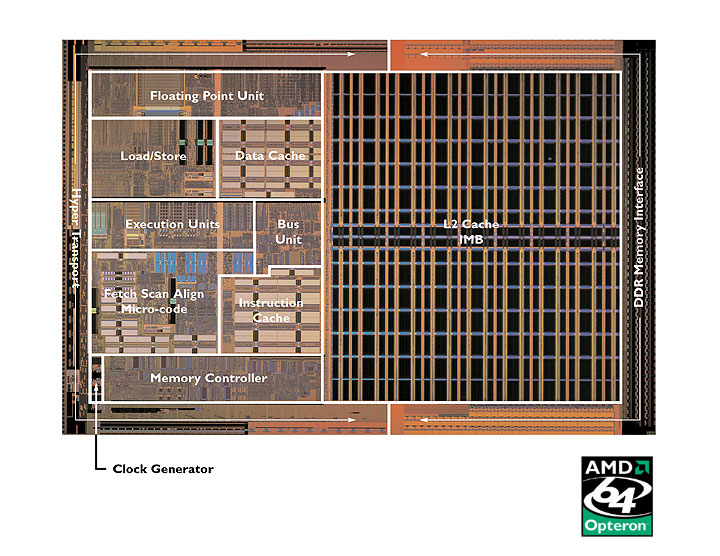
\includegraphics[width=11.25cm]{../caching/Opteron_die_labelled.jpg}};
%\draw[red] (0, 0) grid (9,7);
    \newcommand{\pyrShift}{0.5cm}
\onslide<2->{
    \draw[fill=red,opacity=0.6] (1.9,6.2) rectangle (2.4,5.8);
    \draw[fill=red,opacity=0.6] (1.7,4.2) rectangle (1.9,4.6);

    \begin{scope}[xshift=\pyrShift]
    \draw[fill=red!60!white] (10,7) -- (9.75,6.5) -- (10.25,6.5) -- cycle;
    \node[anchor=west] at (10.1, 6.75) {Registers};
    \end{scope}
}
\onslide<3->{
    %\draw[fill=orange,opacity=0.6] (2.95,2.7) rectangle (4.2,3.6);
    \draw[fill=orange,opacity=0.6] (2.95,2.7) -| (4.2,3.8) -| (3.6,3.65) -- (2.95,3.65) -- (2.95,2.7);
    \draw[fill=orange,opacity=0.6] (2.95,4.6) rectangle (4.2,5.6);

    \begin{scope}[xshift=\pyrShift]
    \draw[fill=orange!60!white] (9.5,6) -- (9.75,6.5) -- (10.25,6.5) -- (10.5,6) -- cycle;
    \node[anchor=west] at (10.35,6.25) {L1 cache};
    \end{scope}
}
\onslide<4->{
    \draw[fill=yellow,opacity=0.6] (4.2,2.1) rectangle (7.9,6.25);
    
    \begin{scope}[xshift=\pyrShift]
    \draw[fill=yellow!60!white] (9.25,5.5) -- (9.5,6) -- (10.5,6) -- (10.75,5.5) -- cycle;
    \node[anchor=west] at (10.6,5.75) {L2 cache};
    \end{scope}
}
\onslide<6->{
    \begin{scope}[xshift=\pyrShift]
    \draw[pattern color=green!60!white,pattern=north west lines] (9.0,5.) -- (9.25,5.5) -- (10.75,5.5) -- (11.,5.) -- cycle;
    \node[anchor=west] at (10.85,5.25) {L3 cache};
    \draw[fill=blue!60!white] (8.5,4.) -- (9.,5.) -- (11,5.) -- (11.5,4.) -- cycle;
    \node[anchor=center,align=center] at (10.,4.5) {main\\memory};
    \end{scope}
}
\onslide<7->{
    \begin{scope}[xshift=\pyrShift]
    \fill[white,opacity=0.9] (7.0,4.5) rectangle (8.4,10.0);
    \begin{scope}[font=\fontsize{10}{11}\selectfont]
        \node[anchor=east] at (9.,6.75) {$<1$ ns};
        \node[anchor=east] at (9.,6.25) {$\sim1$ ns};
        \node[anchor=east] at (9.,5.75) {$\sim5$ ns};
        \node[anchor=east] at (9.,5.25) {$\sim20$ ns};
        \node[anchor=east] at (9.,4.75) {$\sim100$ ns};
    \end{scope}
    \end{scope}
}
\end{tikzpicture}
    \imagecredit{Image: approx 2004 AMD press image of Opteron die; \\ approx register location via chip-architect.org (Hans de Vries)}
\end{frame}



\section{instruction-level parallelism}

\begin{frame}[fragile]{some performance examples}
\begin{tikzpicture}
\node[draw,very thick,align=left] (v1) {
\lstset{language=myasm,style=smaller,morekeywords={decq}}
\begin{lstlisting}
example1:
    movq $10000000000, %rax
loop1:
    addq %rbx, %rcx
    decq %rax
    jge loop1
    ret
\end{lstlisting}
};
\node[align=left,anchor=north] at (v1.south) {
\myemph<2>{about 30B} instructions \\
my desktop: approx \myemph<2>{2.65 sec}
};
\node[align=left,draw,very thick,anchor=north west] (v2) at ([xshift=1cm]v1.north east) {
\lstset{language=myasm,style=smaller,morekeywords={decq}}
\begin{lstlisting}
example2:
    movq $10000000000, %rax
loop2:
    addq %rbx, %rcx
    addq %r8, %r9
    decq %rax
    jge loop2
    ret
\end{lstlisting}
};
\node[align=left,anchor=north] at (v2.south) {
\myemph<2>{about 40B} instructions \\
my desktop: approx \myemph<2>{2.65 sec}
};
\end{tikzpicture}
\end{frame}


\section{C review}
\begin{frame}[fragile]{C exercise}
\lstset{language=C,style=small}
\begin{lstlisting}
int array[4] = {10,20,30,40};
int *p;
p = &array[0];
p += 2;
p[1] += 1;
\end{lstlisting}
array = \\
\begin{tabular}{llll}
    A. & compile or runtime error   & B. & \{10,20,30,41\} \\
C. & \{10,20,32,41\} & D. & \{10,21,30,40\} \\
E. & \{12,21,30,40\} & F. & none of these \\
\end{tabular}
\end{frame}

\begin{frame}<1>[fragile,label=cExer2]{C exercise (2)}
\lstset{language=C,style=smaller}
\begin{lstlisting}
int *array2[4]; int array1[4] = {10,20,30,40};
void mystery(int **p) {
    *p = &array1[2];
}
int main() {
    int **q;
    q = array2;
    mystery(q);
    array1[1] = *q;
    ...
}
\end{lstlisting}
array1 = \\
\begin{tabular}{llll}
\myemph<2>{A.} & compile or runtime error   & B. & \{10,10,30,40\} \\
C. & \{10,30,30,40\} & D. & \{10,10,20,30\} \\
E. & \{10,20,10,20\} & \myemph<2>{F.} & none of these \\
\end{tabular}
\end{frame}

\iftoggle{heldback}{}{\againframe<2>{cExer2}}


\usetikzlibrary{shapes.misc}

\begin{frame}{some pointer stuff}
\begin{tikzpicture}
\begin{scope}[y=0.9cm]
\draw (0, 0) rectangle (4, -8);
\foreach \x/\v in {0/0x040,1/0x038,2/0x030,3/0x028,4/0x020,5/0x018,6/0x010,7/0x008,8/0x000} {
    \node[font=\tt,anchor=east] at (0, -\x) {\v};
}
\node[anchor=north west, overlay,font=\tt,align=left] (decl p) at (4.2, 1) {
\texttt{int array[2]=}\texttt{\{0x12,0x45,0x67\};} \\
\texttt{int single = 0x78;} \\
\texttt{int *ptr;} \\
\alt<6>{ptr = \&single; \\ }{\alt<9>{ptr = \&array[0]; \\}{}}
};
\begin{visibleenv}<3>
\node[cross out,draw=red,very thick,font=\tt,anchor=north west] (bad ptr) at (decl p.south west) {
*ptr = 0xAB;
};
\node[right] at (bad ptr.east) {compile error};
\end{visibleenv}
\begin{visibleenv}<4-5>
\node[very thick,align=left,font=\tt,anchor=north west] (ptr single) at (decl p.south west) {
\myemph<4>{ptr = \&single;} \\
\myemph<4>{ptr = (int*) 0x28;} {\scriptsize\normalfont addr. of single} \\
};
\begin{visibleenv}<5>
\node[cross out,draw=red,very thick,font=\tt,anchor=north west] (bad ptr single) at (ptr single.south west) {
ptr = 0x28;
};
\node[right] at (bad ptr single.east) {compile error};
\node[cross out,draw=red,very thick,font=\tt,anchor=north west] (bad ptr single 2) at ([yshift=-.25cm]bad ptr single.south west) {
ptr = (int*) single;
};
\node[below,align=left] at (bad ptr single 2.south) {pointer to unknown place};
\end{visibleenv}
\end{visibleenv}
\begin{visibleenv}<6>
\node[very thick,align=left,font=\tt,anchor=north west] (ptr set) at (decl p.south west) {
\myemph<6>{*ptr = 0xFF;} 
};
\end{visibleenv}
\begin{visibleenv}<7-8>
\node[very thick,align=left,font=\tt,anchor=north west] (ptr single) at (decl p.south west) {
\myemph<4>{ptr = array;} \\
\myemph<4>{ptr = \&array[0];} \\
\myemph<4>{ptr = (int*) 0x2C;} \\
};
\begin{visibleenv}<8>
\node[cross out,draw=red,very thick,font=\tt,anchor=north west] (bad ptr single) at (ptr single.south west) {
ptr = array[0];
};
\node[right] at (bad ptr single.east) {compile error};
\node[cross out,draw=red,very thick,font=\tt,anchor=north west] (bad ptr single 2) at ([yshift=-.25cm]bad ptr single.south west) {
ptr = (int*) array[0];
};
\node[below,align=left] at (bad ptr single 2.south) {pointer to unknown place};
\end{visibleenv}
\end{visibleenv}
\begin{visibleenv}<9>
\node[very thick,align=left,font=\tt,anchor=north west] (ptr set) at (decl p.south west) {
\myemph{ptr[2] = 0xFF;} \\
\myemph{*(ptr + 2) = 0xFF;} \\
~ \\
int *temp1; temp1 = ptr + 2; \\ \myemph{*temp1 = 0xFF;} \\
~ \\
int *temp2; temp2 = \&ptr[2]; \\ \myemph{*temp2 = 0xFF;} \\
};
\end{visibleenv}
\begin{visibleenv}<10>
\node[very thick,align=left,font=\tt,anchor=north west] (by ptr pattern) at (decl p.south west) {
void change\_arg(int *x) \{ \\
\hspace{1cm} *x = compute\_some\_value(); \\
\} \\
\ldots \\
change\_arg(\&single); 
};
\end{visibleenv}
\begin{visibleenv}<2->
\begin{scope}[every node/.style={font=\tt\small}]
    \draw[alt=<9>{fill=red!10}] (0, -1.5) rectangle (4, -1) node[midway]{\alt<9>{array[2]: 0xFF}{array[2]: 0x67}};
    \draw[] (0, -2) rectangle (4, -1.5) node[midway]{array[1]: 0x45};
    \draw[] (0, -2.5) rectangle (4, -2) node[midway]{array[0]: 0x12};
    \draw[alt={<6,10>{fill=red!10}}] (0, -3) rectangle (4, -2.5) node[midway]{\alt<10>{single: \ldots}{\alt<6>{single: 0xFF}{single: 0x78}}};
    \draw[alt=<4>{fill=red!10}] (0, -4) rectangle (4, -3) node[midway]{%
        \alt<7->{ptr: 0x2C}{\alt<4->{ptr: 0x28}{ptr = ???}}%
    };
\end{scope}
\end{visibleenv}
\end{scope}
\end{tikzpicture}
\end{frame}

\begin{frame}{some avenues for review}
    \begin{itemize}
    \item review CSO1 stuff
        \begin{itemize}
        \item labs 9--12 (of last Spring)
        \item \url{https://www.cs.virginia.edu/~jh2jf/courses/cs2130/spring2023/}
        \end{itemize}
    \item exercises we've used in the past:
        \begin{itemize}
        \item implement strsep library function
        \item implement conversion from dynamic array to linked list
        \end{itemize}
    \end{itemize}
\end{frame}

